\chapter{Summary and Conclusions}
\label{chapter:summary}
\section{Summary}
\renewcommand{\arraystretch}{1.2}
\begin{table}
    \begin{center}
\begin{tabular}{|>{\centering\arraybackslash}m{3.5cm}|>{\centering\arraybackslash}m{3.0cm}|>{\centering\arraybackslash}m{4.5cm}|}
\hline
Depth-cue & Volumetric AR display & Varifocal-occlusion AR display \\
\hline
Accommodation & All depths & Selectable depth \\
\hline
Retinal blur & Natural & Synthetic \\
\hline
Occlusion & None & Depth-dependent and Hard-edge \\
\hline
\end{tabular}
    \end{center}
\caption[Summary of contributions]{Summary of contributions}
\label{tab:summary_contributions}
\end{table}

This dissertation was motivated by the lack of perceptually realistic depth cues in the current generation commercial augmented reality displays and research prototypes. This dissertation focuses on three particularly important depth cues, namely, accommodation, defocus blur, and mutual occlusion. We presented two augmented reality displays which present high-quality accommodation, defocus blur, and occlusion across a large depth-range.

\emph{Volumetric AR display}, is a multifocal display with 280 single-color binary image planes – a significant improvement upon previous multifocal displays. The volumetric AR display can present full-color imagery (24 or higher bit-depth) spanning a large volume (15 cm to 400 cm with $45^\circ$ Field-of-View) composed of 280 binary images, each of which has the native resolution of the display ($1024 \times 768$). This dissertation discusses the optical design, synchronization electronics, and the graphics rendering pipeline. One of the stages of the graphics rendering pipeline is the decomposition of the color-volume to the binary-volume. This dissertation develops multiple decomposition schemes --- one fixed-pipeline decomposition and multiple optimization-based methods. While most of the results were obtained using an offline implementation of the graphics rendering pipeline, a simple real-time system composed of 8 single-color binary image planes was implemented and was demonstrated with a video recording. 

\emph{Varifocal occlusion display}, is an extension of fixed-focus occlusion displays, and enables a single occlusion image plane to be moveable in depth. This dissertation asserts that extending fixed-focus occlusion displays to varifocal occlusion displays requires a solution to the following problem: that the tunable optics needed to move the occlusion/virtual image plane in depth also needs to transmit the image of the real-world undistorted. To solve this problem, this dissertation analyses the problem using concepts of light fields and uses ray-transfer matrix equations to derive optical designs using optimization and analytical derivation. A real-time system was built using off-the-shelf components and used to compare the proposed technology to previous AR display technologies.

Table 5.1 quantitatively compares the nature and performance of this dissertation’s displays against the monocular depth cues considered here. 

\section{Future Work}
The immediate next research steps for the volumetric NED could be the real-time implementation of the proposed rendering pipeline. 
This is not a trivial improvement because of the large computation and communication demands that the system needs to address. 
However, addressing this large computation and communication demand should be possible with this NED because its components were originally designed for a low-latency AR display~\cite{Lincoln2016motion}. 
So, in addition to a real-time volumetric NED, future work could include developing a low-latency volumetric NED. 

The ability of our varifocal occlusion-capable AR display to attenuate real-world light can also be used to depict consistent global-illumination in the AR scene and depict interesting effects such as shadows cast by virtual objects onto the real world and vice-versa, or to relight the real-world to match the virtual scene.
The bulky form-factor of image-forming occlusion displays remains the key limitation, and addressing this is definitely an area for future work. 

Both of the presented display technologies can also emulate multiple other AR displays, e.g., the volumetric NED can also emulate previous varifocal NEDs and previous multifocal NEDs, and the varifocal occlusion-capable NED can also emulate fixed-focus occlusion displays and occlusion incapable varifocal AR displays. 
Hence, this dissertation’s displays could be used as test-beds to conduct perceptual experiments to understand the human visual system better and to come up with strategies for future NEDs.

\section{Conclusion}
\begin{figure}[h!]
\centering
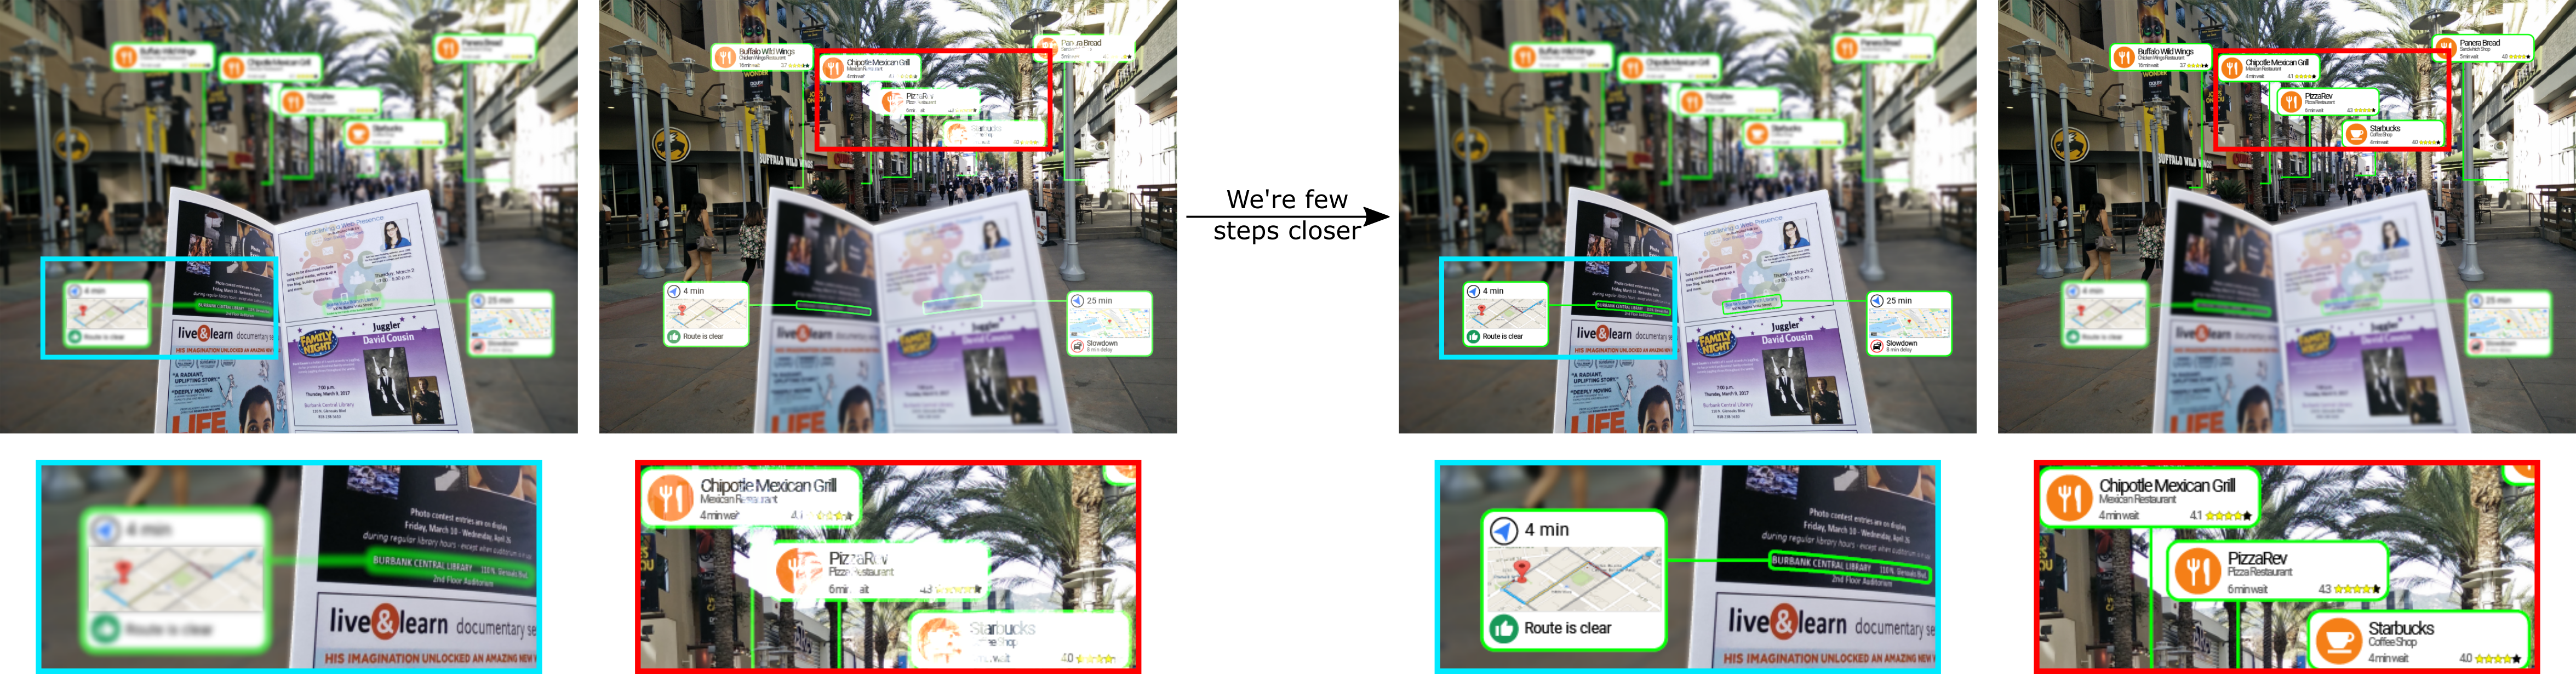
\includegraphics[width=0.99\columnwidth]{images/other/contributions}
\caption[Contributions of this dissertation]{Figures shows the contributions of this dissertation with a concept diagram. We've take small steps to go from the current state-of-the-art (on the left) to the envisioned future for augmented reality displays (on the right). Insests at the bottom row show enlarged portions of the regions of interest in the concept image above them. Image credit: Adapted from David Dunn.}
\label{fig:contributions}
\end{figure}


Fig.~\ref{fig:contributions} shows a concept augmented reality scene. In this concept scene, the real scene is composed of a pamphlet in the foreground and shops and restaurants in the background. To this scene, the current generation augmented reality displays can superimpose a transparent image at a fixed distance. However, the ultimate display as envisioned for augmented reality will be able to display multiple images at their correct depths with perceptually consistent depths. This dissertation takes a few steps towards realizing this vision.

\myblockquote{
The screen is a window through which one sees a virtual world. The challenge is to make that world look real, act real, sound real, feel real.
}{\cite{sutherland1965ultimate}}

Although the above quote is intended for Virtual Reality and considers multiple modalities (sight, hearing, haptics), it helps to convey the vision for Augmented Reality that I subscribe to. 
The ultimate Augmented Reality display would combine the real and the virtual worlds in a visually convincing manner—with consistent depth cues, latency, resolution, color fidelity, lighting, shadows, reflections, etc. 
Towards realizing this vision, this dissertation develops methods to improve monocular depth cues for Augmented Reality displays. 

